\documentclass[usenames,dvipsnames]{beamer}
\usepackage{braket}
\usepackage{xcolor}
\usepackage{amsmath}
\usepackage{amsfonts}
\usepackage{tikz}
\usepackage{adjustbox}
\usepackage{subcaption}
\usepackage{svg}
\usepackage{graphicx}
\usepackage{media9}
\usepackage{float}
\usetikzlibrary{calc}
\usepackage{array}
\usepackage{efbox,graphicx}
\usepackage[normalem]{ulem}
\usepackage[dvipsnames]{xcolor}


\efboxsetup{linecolor=\color{OliveGreen},linewidth=1pt, margin=0.1pt}



\usetheme{EastLansing}
\title[Building A Computer Without A Computer] % (optional, only for long titles)
{Building A Computer Without A Computer.}
\subtitle{ ( Introduction To Error Crorrection And Fault Tolarnce Computation. ) }
\author[D.~Ponarovsky] % (optional, for multiple authors)
	{D.~Ponarovsky\inst{1}}

\institute[HUJI] % (optional)
	{ \inst{1} Faculty of Computer Science\newline
	  Hebrew University of Jerusalem
	}
\date[2022-23] % (optional)
{Qubit meeting 2022-23, Israel Quntum Tech Community.}
\subject{Quantum Error Correction}

\begin{document}
\usebackgroundtemplate{%             declare it
\tikz[overlay,remember picture] \node[opacity=0.4, at=(current page.center)] {
   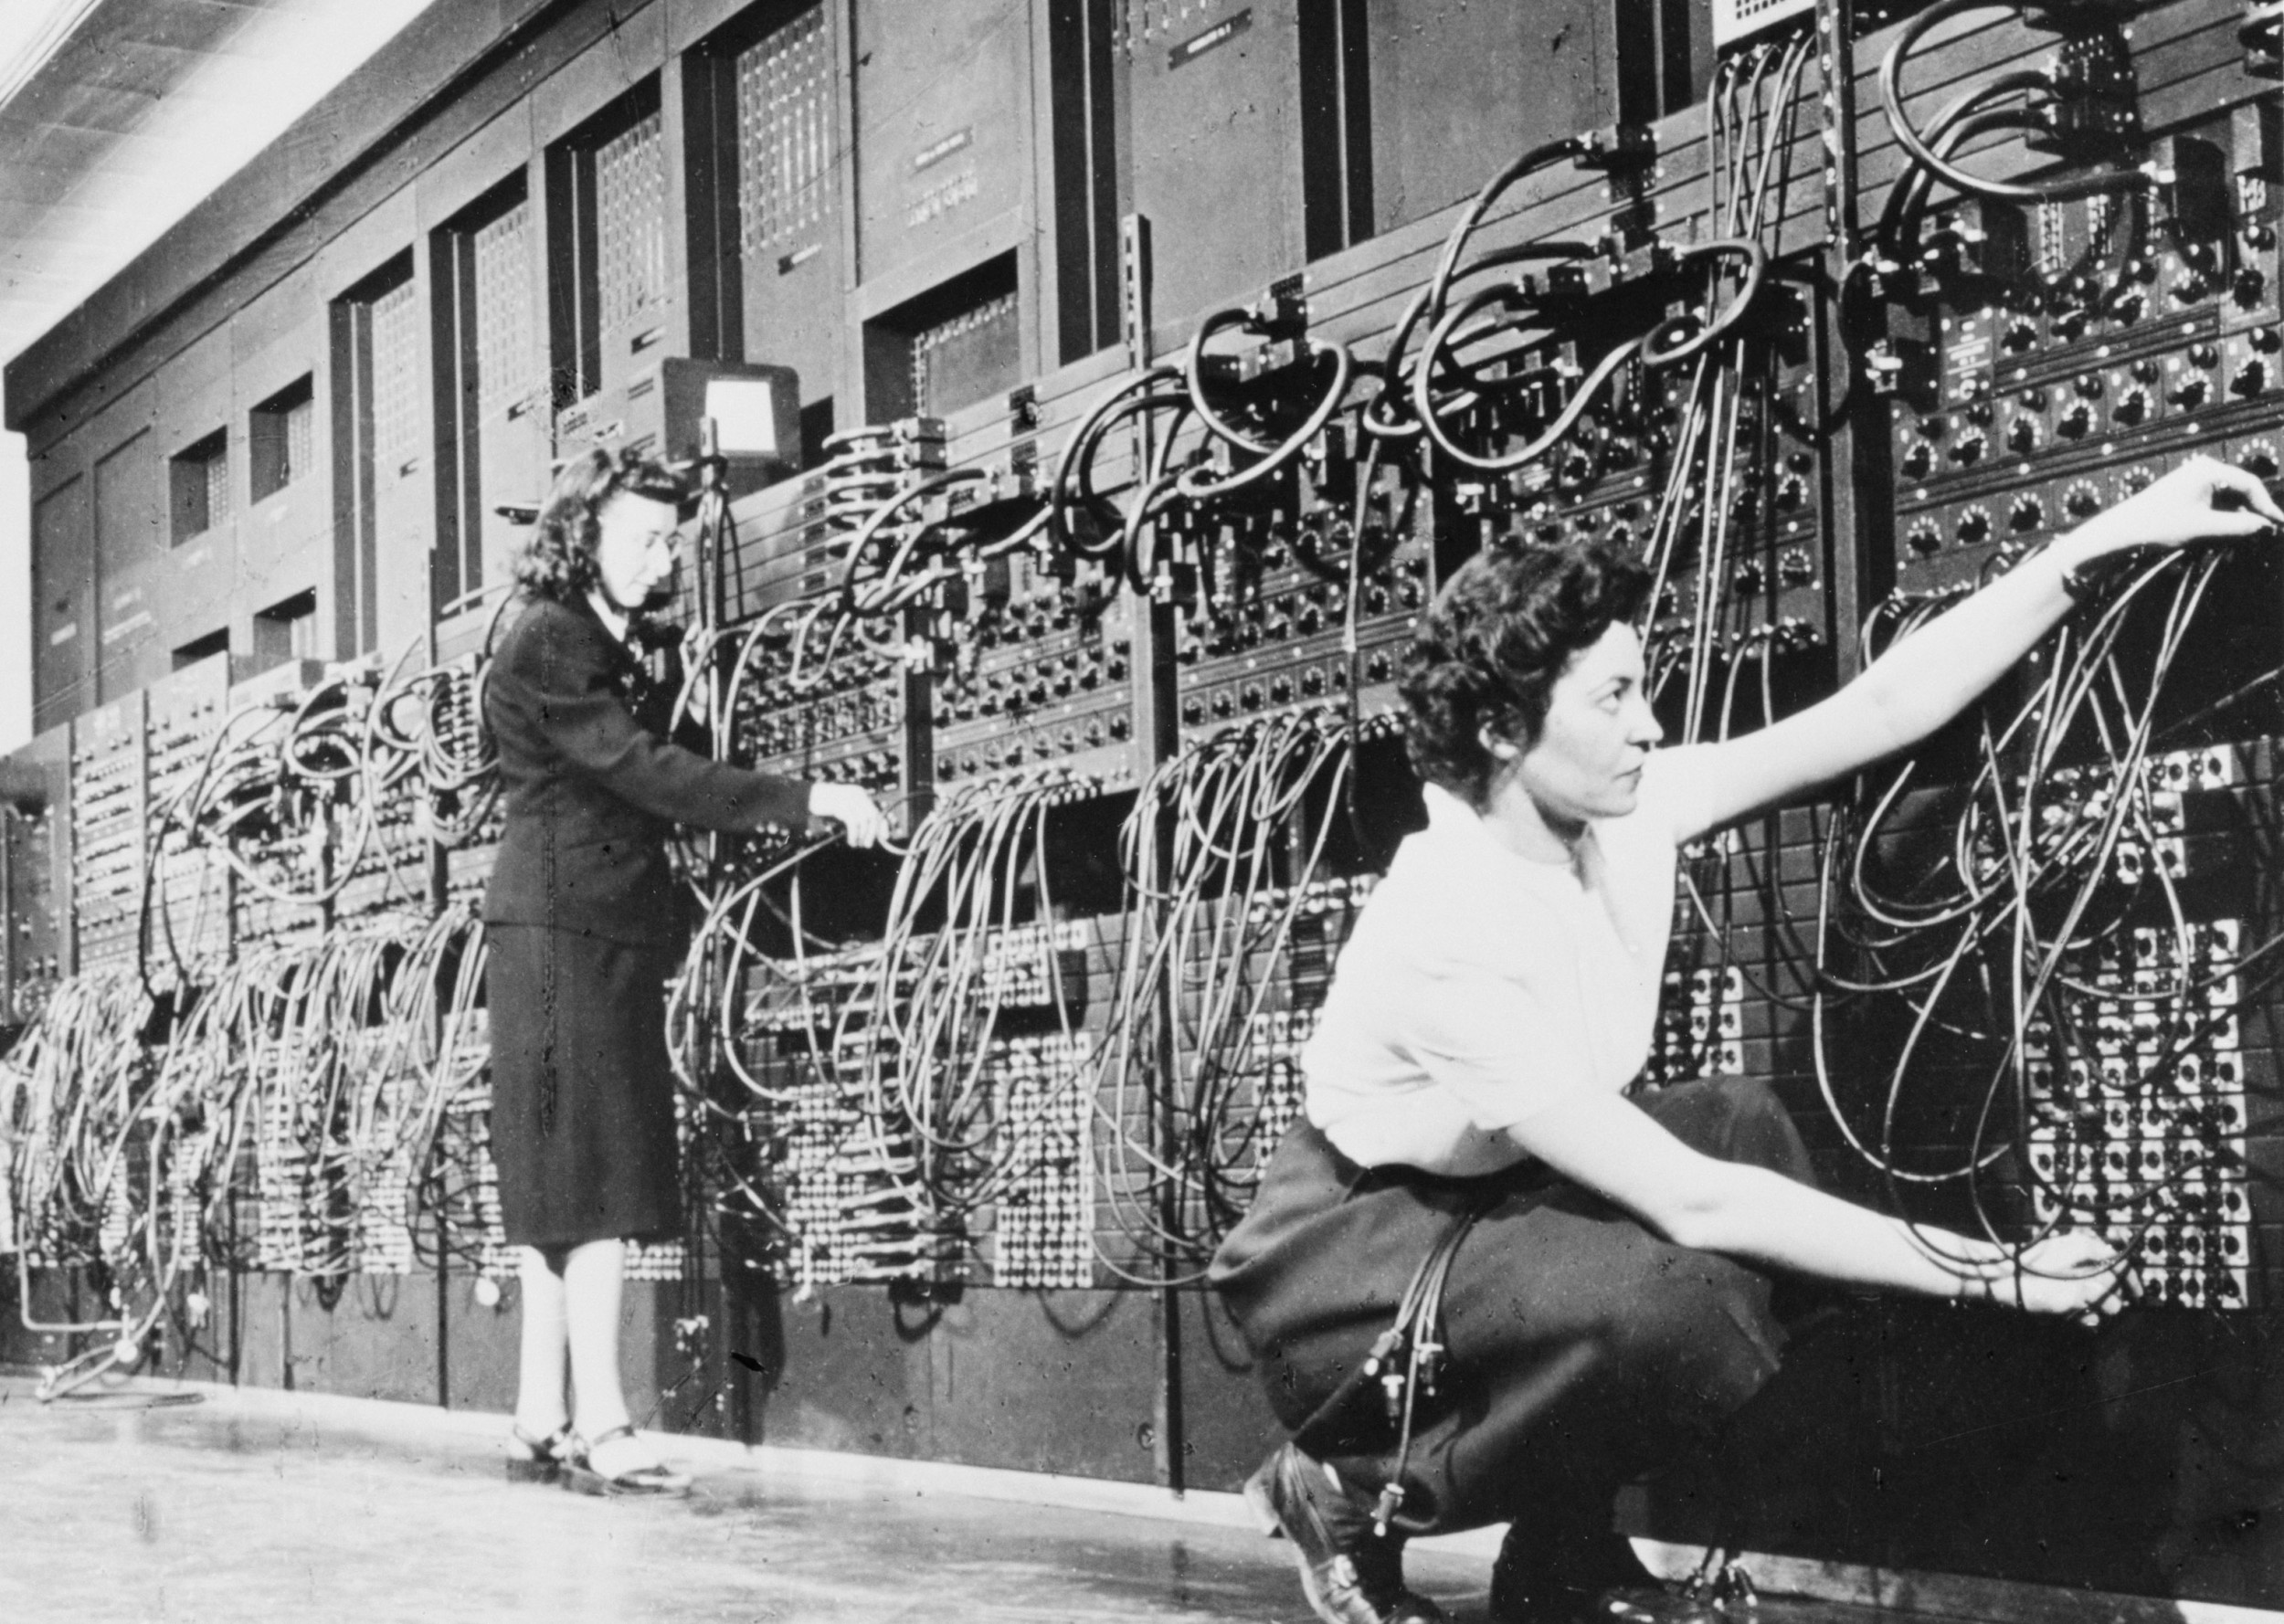
\includegraphics[height=\paperheight,width=\paperwidth]{1260_original.jpg}};
}

     \begin{frame}
     \maketitle
   \end{frame}

   \begin{frame}
     \frametitle{ The Goal Of The Talk  }

   \begin{exampleblock}{ Blocktitle } 
     \begin{itemize}
       \item<1-> Motivation. Answer on what we are fighting for. Give a non-cryptogriphc advantage of quantum computing.  
       \item<2-> Reviwing the current status and latest results. Sharing the view of the errors correcion scientist.    
       \item<3-> Engaging. Build a common language, explain all the frighting terms (Noise, Tresholds, NISQ, Advantage). Talking Buisness. 
    \end{itemize}
  \end{exampleblock}
   \end{frame}
	\section{Motivation}
	\begin{frame}[t]
	\frametitle{Motivation.}
	 
	\begin{exampleblock}{The Question.}
	    Why should we have a \only<1>{Quantum} \uncover<2-> {\sout{Quantum} Classic} Computer?
	  \end{exampleblock}

	  \uncover<3->{ 
	    \efbox{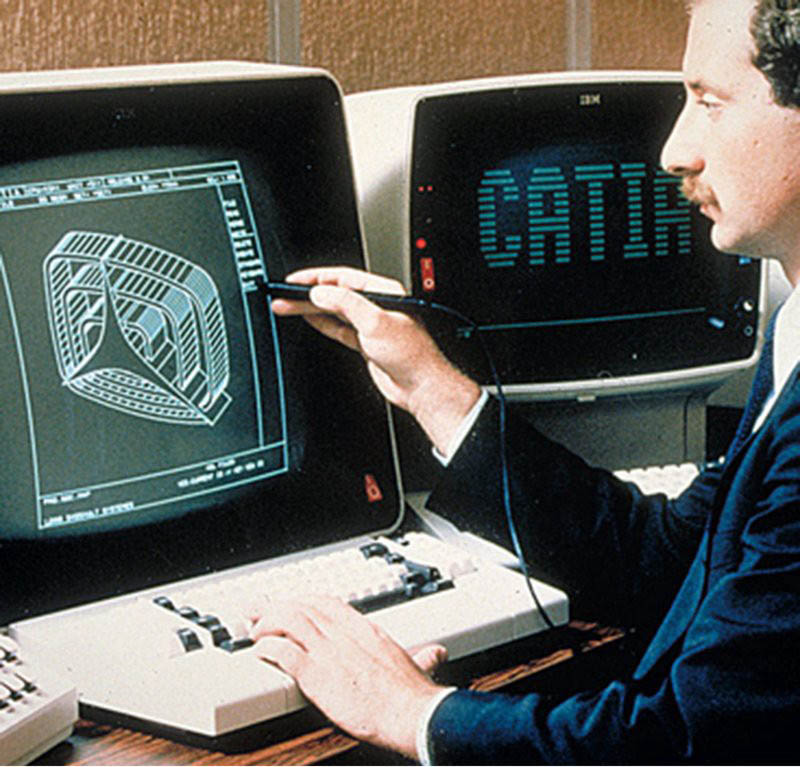
\includegraphics[height=100pt,width=120pt]{rsut6ggvivt81.jpg}}
	  }
	  
	  \uncover<4-> {
	    \vspace*{-3cm} \hspace*{6cm}  \efbox{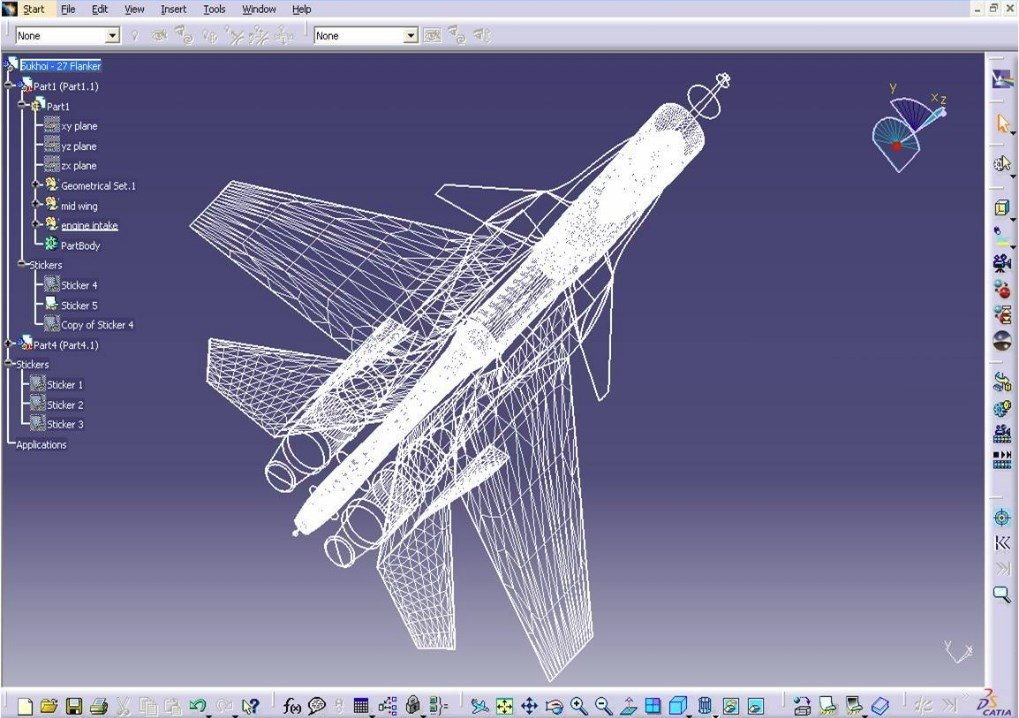
\includegraphics[height=150pt,width=120pt]{catia-21987-5.jpg}}
	  }
	  
	  \uncover<5-> {
	    \vspace*{-3cm} \hspace*{2cm}  \efbox{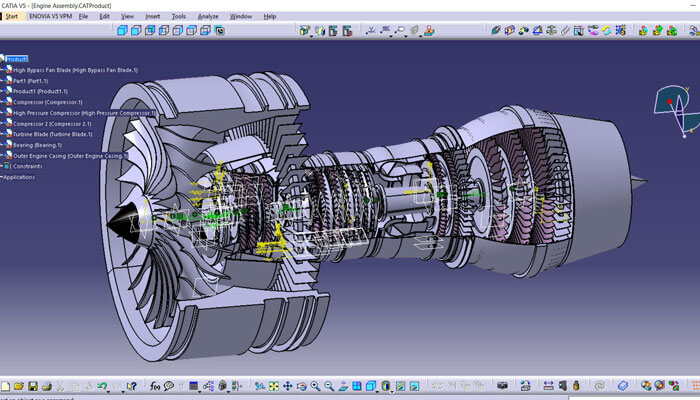
\includegraphics[height=80pt,width=100pt]{what-is-catia-051120.jpg}}
	  }
     
	\end{frame}


	\begin{frame}
		\uncover<1-> {
	    		\vspace*{-3cm} \hspace*{6cm}  \efbox{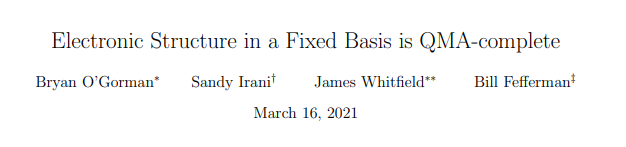
\includegraphics[resolution=1111111111100]{QMA-com.png}}
	  	}
	  
	  	\uncover<2-> {
	    		\vspace*{-3cm} \hspace*{2cm}  \efbox{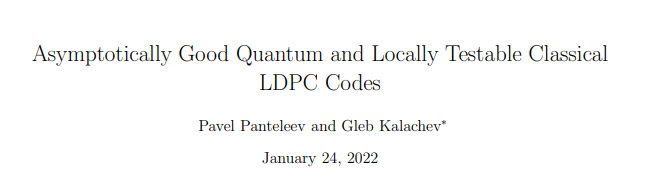
\includegraphics[height=80pt,width=200pt]{QLPDC.png}}
	  	}
	\end{frame}


\usebackgroundtemplate{ }    %% undeclare it
     \section{About}
	\begin{frame}
	  \frametitle{ About this Presention.  }
	   \begin{columns}[T] % contents are top vertically aligned
     \begin{column}{.23\textwidth} % each column can also be its own environment
     Contents of first column \newline split into two lines
     \end{column}
     \begin{column}{.23\textwidth} % each column can also be its own environment
     Contents of first column \newline split into two lines
     \end{column}
     \begin{column}{.23\textwidth} % each column can also be its own environment
     Contents of first column \newline split into two lines
     \end{column}
     \begin{column}{.23\textwidth} % alternative top-align that's better for graphics
     Contents of first column \newline split into two lines
          %\includegraphics[height=3cm]{graphic}
     \end{column}
     \end{columns}
	\end{frame}
	\begin{frame}
	  \frametitle{ Sounds Grate, Whats is the catch? }
		here you can put any text/equation etc. 
		$a^2 + b^2 = c^2$.		
	\end{frame}\begin{frame}
	  \frametitle{ Wait a minute. }
		here you can put any text/equation etc. 
		$a^2 + b^2 = c^2$.		
	\end{frame}
	\begin{frame}
		\frametitle{This is the second slide}
		\framesubtitle{A bit more information about this}
		Some random text.		
	\end{frame}
\end{document}
